\chapter{状態表現の階層性を考慮することによる深層状態空間モデルの拡張}
\label{chap:proposal}
を目指す.

はじめに,提案手法で扱う問題設定について整理し,その後提案手法の具体的な説明として,確率モデル・最適化とモデルアーキテクチャについて述べていく.

\section{問題設定}
本研究では行動条件付き映像予測の問題を解く.具体的には、ある行動主体が実行した行動系列$\vec{a}$とその結果観測される観測系列$\vec{o}$のセット$\{\vec{a}, \vec{o}\}$が予め多数与えられたときに、未知の初期状態と行動系列から結果として観測される映像を予測できるようにする.

\section{ベースライン}
本研究では2章で述べたシンプルなDSSMをベースラインにおく.

\section{提案手法}
3章で述べたように、ベースラインは潜在変数の次元を大きくすると学習がうまく行かない.提案手法は,より豊かな状態表現を獲得できるようにするようベースラインのDSSMを拡張することが目的である.

\subsection{状態表現の階層性}
まず、潜在変数の次元を変えた時に獲得される情報について考察する.状態表現学習によって,ベースラインモデルが潜在変数の次元を変えたときに獲得する情報と、潜在変数を高次元にした際に獲得してほしい情報、そしてすべての情報の関係性を考える.

\begin{figure}[tbp]
  \begin{center}
    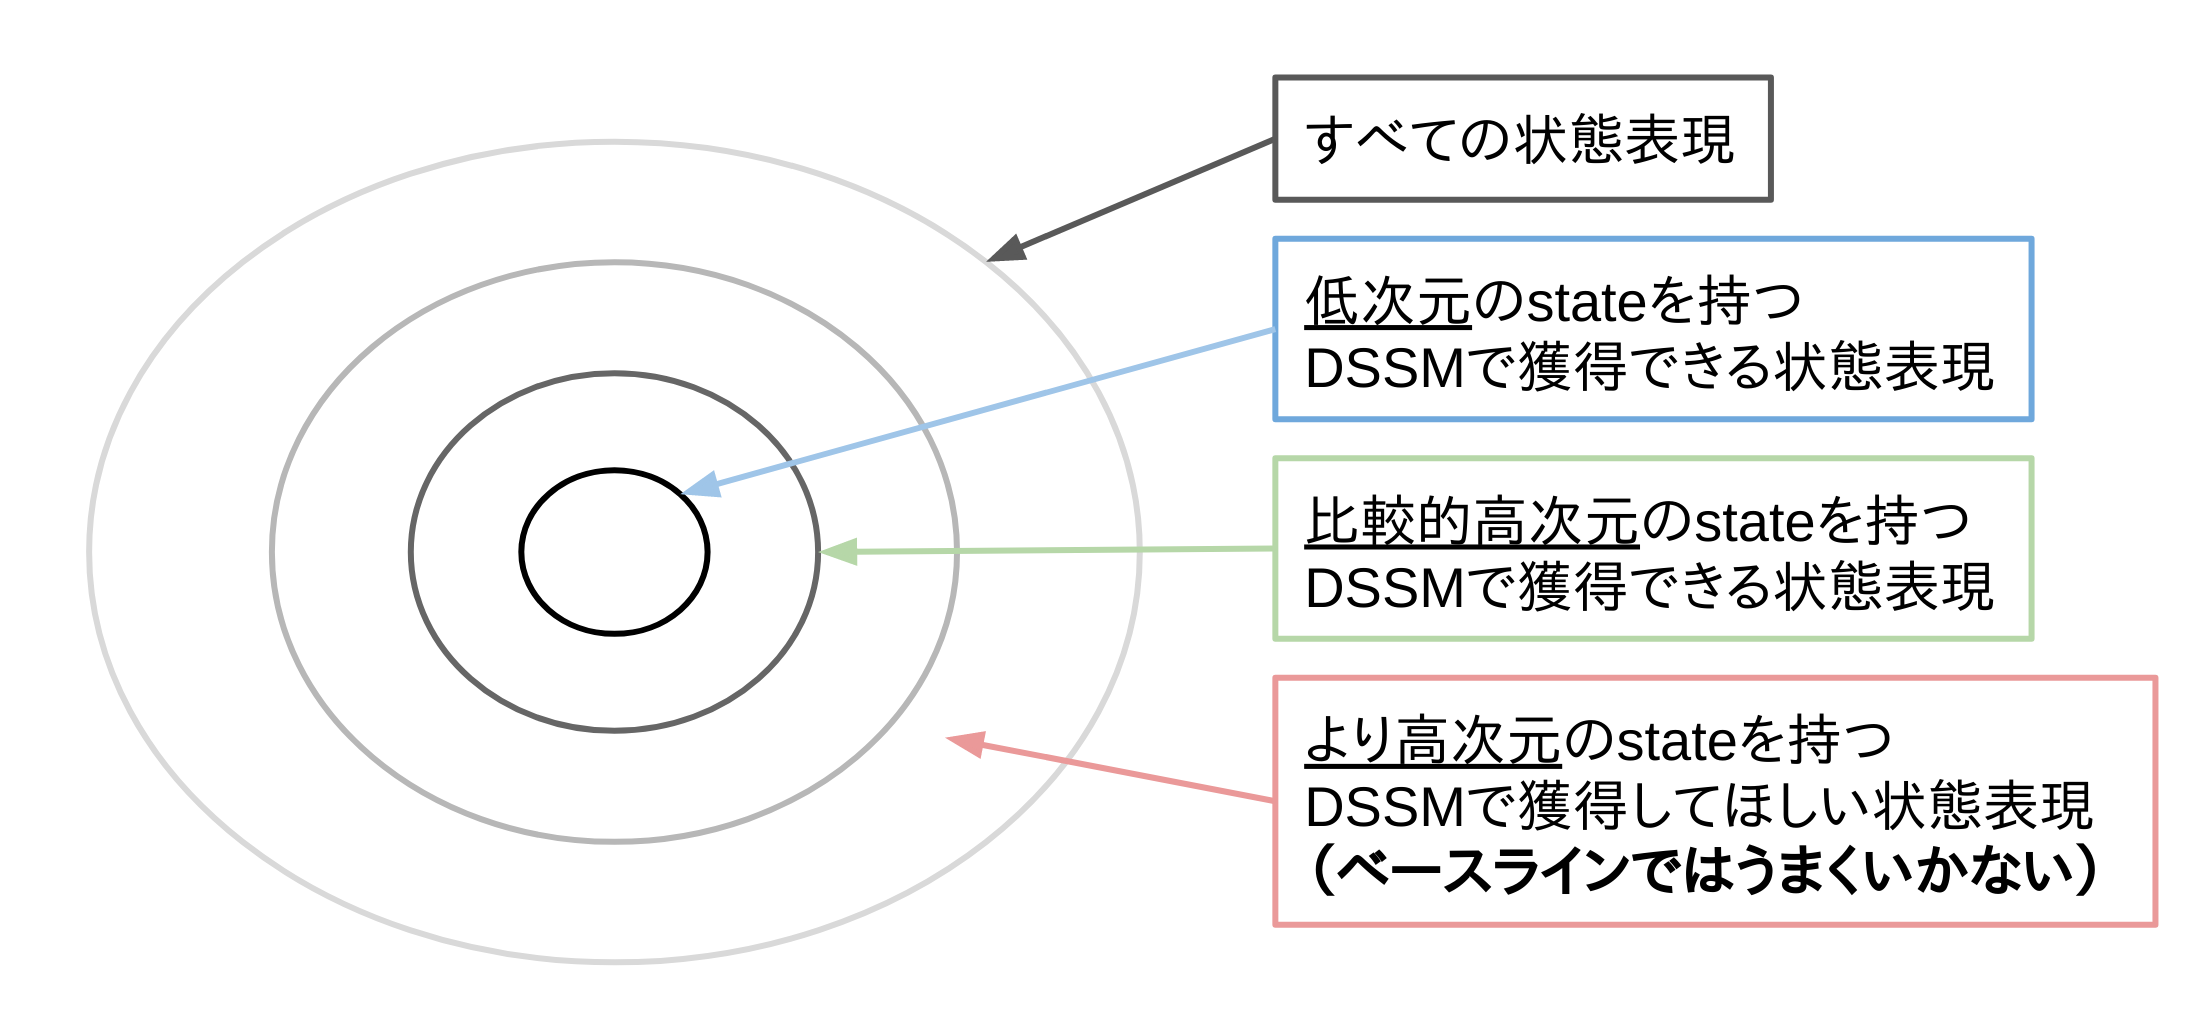
\includegraphics[width=\linewidth]{./figures/hierarchical.png}
    \caption{hierarchical}
    \label{fig:hierarchical}
  \end{center}
\end{figure}


中心的な情報から順に獲得される.
中心的な情報が獲得できないうちに表面的な情報を獲得しても,中心的な表現が間違っていれば生成されるものも異なり,学習時に誤差を小さくできないからである.
というように、現実的なデータの背後にある状態表現には階層性がある.今、低次元であれば
まず背景、次によく動く部分、最後に細かいテクスチャ、という順番に学習されるのが合理的である.つまり、stateの次元を大きくしたときに学習される情報には図のような包含関係がある.

今、

理想的には、stateの次元を徐々に大きくすることである.
ベースラインでは、Fig \ref{fig:hierarchical}の赤で示した部分をいきなり学習しようとするが、


ただし状態表現の外側になるほど得られるデータが疎になるので,表現としては獲得しにくくなる
モデルに正規分布を仮定していることによる表現力の制約などを除けば、

\subsection{階層的な状態表現の遷移}
前節より、状態表現に階層性があることを述べたが,この節では階層的な状態表現の遷移を考える.
遷移にも順序がある.つまり,中心的な状態表現が遷移した後,
更新前を白で、更新後を灰色で表している
ベースラインのDSSMモデルは、提案するHDSSMの特別な場合と解釈することもできる.


\begin{figure}[tbp]
  \begin{center}
    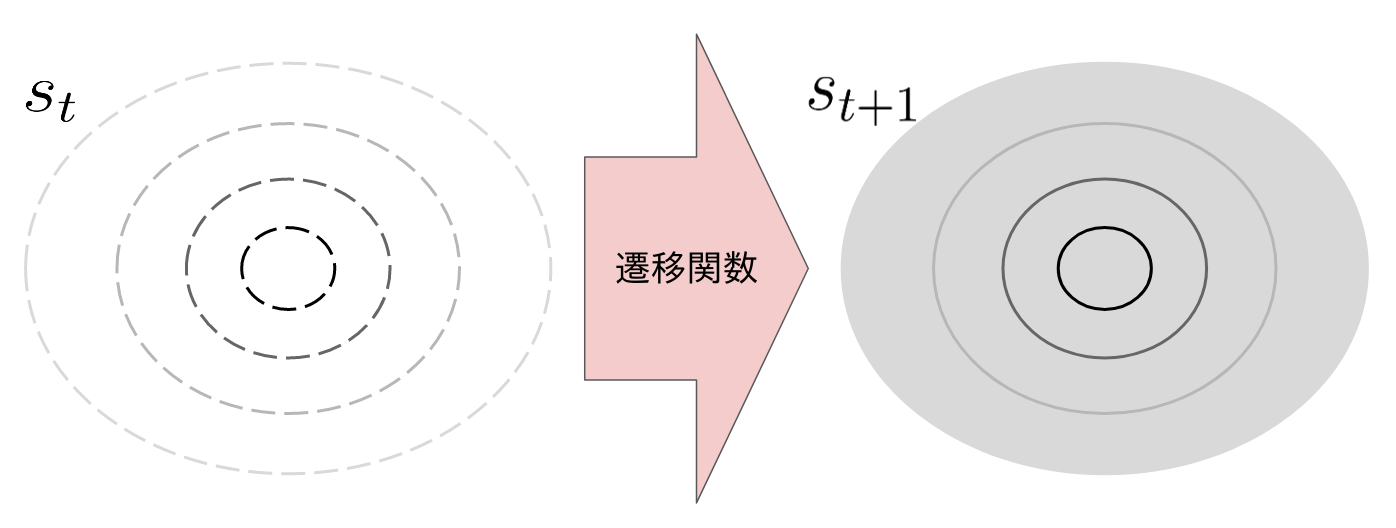
\includegraphics[scale=0.2]{./figures/transition_base.png}
    \caption{transition base}
    \label{fig:transition_base}
  \end{center}
\end{figure}


\begin{figure}[tbp]
  \begin{center}
    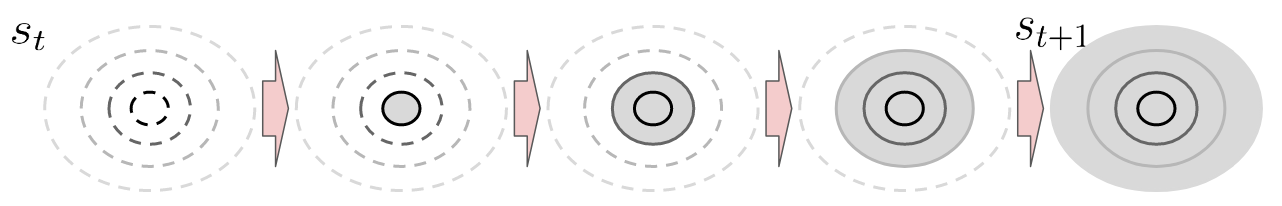
\includegraphics[width=\linewidth]{./figures/transition_proposal.png}
    \caption{transition proposal}
    \label{fig:transition_proposal}
  \end{center}
\end{figure}



\subsection{確率モデル・最適化}

ここまでで、潜在変数の次元を大きくした際に,獲得できる状態表現とその遷移がどのようなものかを考察した.


\subsection{データの生成方法(評価時)}
\section{類似手法との差分}
DRAW[]はVAEの潜在変数に階層性をもたせたモデルで、データに遷移はないが、狙いは提案手法と似ている.多層RNN[]は直前の観測を逐次的に入力すplanetでRNNベースはダイナミクスの獲得が弱く,長期の予測が難しいと報告されている.FHMMは離散低次元でEMアルゴリズムによって最適化をしている

% videoflowはaction conditionalじゃないしー

